\part{Le projet}

\section{Organisation du code}

La plupart des fonctionnalités de notre projet sont encapsulées dans des modules. Ainsi, l'interpréteur \fouine et la machine SECD constituent deux modules que l'on charge dans le fichier main. Nous avons privilégié cette approche pour deux raisons. D'une part par souci de propreté : on minimise le nombre de primitives que l'on peut appeler depuis l'extérieur du module à l'aide des mécanismes de signature (ce qui permet de plus d'inclure de la documentation dans les dites signatures), d'autre part pour rendre le code plus facilement maintenable, dans ce projet où certaines fonctions ont été réécrites plusieurs fois.

\subsection{Liste des fichiers}

\begin{description}
 \item[$\bullet$ main.ml :] Fichier principal. Lit les argument envoyés au programme et fait les différents appels aux différentes parties du code.
 \item[$\bullet$ fouine\_type.ml] Fichier contenant les définitions des types représentant un programme \fouine dans Caml.
 \item[$\bullet$ interpreteur.ml :] Le fichier contenant le module au coeur de \fouine. Contient ma grosse fonction d'interprétation d'un programme \fouine, la fonction \texttt{debug}, qui permet d'afficher un programme \fouine parsé, ainsi que de quoi réaliser l'exécution mixte.
 \item[$\bullet$ machine.ml :] Module implémentant la machine à pile.
 \item[$\bullet$ environnement.ml] La définition du module \texttt{Environnement}, construit à l'aide d'un dictionnaire.
 \item[$\bullet$ dictionnaire.ml] La classe de dictionnaire utilisée. Basée sur une table de hachage.
 \item[$\bullet$ lexParInterface.ml :] Fichier faisant l'interface entre les parser et le reste du code. Fournit simplement des primitives \texttt{read\_prgm <fichier>}.
 \item[$\bullet$ parser.mly , lexer.mll] Ces fichiers permettent de lire la formule donnée en entrée par le programme, et de construire un objet de type programme représentant le code à exécuter.
 \item[$\bullet$ parsMachine.mly , lexMachine.mll] Ces fichiers permettent de lire les instructions donnée en entrée par le programme, et de construire un objet de type \texttt{instruction list} représentant le code à exécuter sur la machine à pile.
\end{description}

\subsection{Liste des programmes \fouine donnés en exemple}

\begin{itemize}
 \item exemples simples sur les différentes fonctionnalités de \fouine (les noms des programmes sont a priori explicites)
 \item fibonacci récursif stupide
 \item fibonacci en temps linéaire avec références
 \item factorielle
 \item tours de Hanoi
 \item crible d'erathosthène (illustration des tableaux)
\end{itemize}

\subsection{Bugs détectés et non corrigés}

\begin{itemize}
 \item la traduction d'environnement \fouine vers SECD suppose qu'une fonction est récursive. Du coup quelquechose défini par
\texttt{let f x = x in let f x = f x in f 2} ne s'exécutera pas correctement, il bouclera au lieu de renvoyer 2.    
\end{itemize}



\section{L'interpréteur \fouine} % section à remplir par Guillaume

\subsection{L'interprétation}

\paragraph{} L'interprétation est réalisée dans la fonction execute du fichier \texttt{interpreteur.ml} . Cette fonction prend en argument un programme \fouine parsé (de type programme) et renvoie un entier. On utilise une fonction récursive auxiliaire qui associe une valeur de type \texttt{ret} au programme. Ensuite, on appelle la petite fonction \texttt{return} qui renvoie un \texttt{int} à partir de ce \texttt{ret}.

\paragraph{} Ce type intermédiaire \texttt{ret} est nécessaire pour pouvoir utiliser des fonctions dans les programmes \fouine. C'est le type des éléments qui sont associés à nos programmes dans l'environnement (\texttt{Env.elt}). Cela permet de renvoyer en interne autre chose que des entiers (ce qui est nécessaire pour les références et les fonctions). De plus, un filtrage par motif dans la fonction return permet de détecter les erreurs dynamiques (entier + fonction) ou (entier + ref) et d'obtenir des messages explicites.

\subsection{Structures de données}

\paragraph{} On utilisera des tables de hachage (Hastbl) qui associeront une valeur \texttt{Env.elt} à une valeur \texttt{programme}. Cette structure de donnée a le gros avantage de gérer parfaitement la portée des variables. En effet, d'après la documentation de Ocaml, lorsqu'une valeur y est assignée à la variable x dans une Hashtbl, l'ancienne valeur de x est remplacée par y. Lorsque l'on supprime l'association (x,y) dans la table, l'ancienne valeur associée à x est restaurée, ce qui est le comportement attendu.

\paragraph{} Cette structure de donnée supporte l'ajout d'un couple d'élément, la suppression d'un élement et de son association (avec éventuelle restauration de la précédente association), la recherche d'un élement et la copie (pour pouvoir faire des clotures).

\paragraph{} Le module \texttt{Environnement} contient de plus la fonction \texttt{transform\_env}, qui transforme l'environnement de l'interpréteur en un environnement lisible par la machine à pile.

\subsection{Fonctions et fonctions récursives}

\paragraph{} Pour l'implémentation des fonctions, on a ajouté un constructeur \texttt{Cloture} au type \texttt{Env.elt}.  Un cloture comprend l'expression de la fonction (le A de \texttt{let f x = A in}) et une copie de l'environnement au moment de la définition de la fonction. Cette copie est "brutale" : on copie l'intégralité de l'environnement sans chercher à savoir quelles valeurs sont inutiles.

\paragraph{} Dans le cas des fonctions récursives, on ajoute à la clôture crée... elle-même. Ainsi, on évite de faire autant de clôtures que d'appel récursif. Cela ne pose pas de problème tant qu'il existe un cas de sortie à la fonction récursive.


\subsection{Les exceptions}

\paragraph{} Les exceptions sont gérées grâce à l'ajout d'un booléen au type de retour de l'interpréteur. Ce booléen vaut vrai si une exception a été levée durant l'éxecution d'un bout de programme. Ainsi, seule l'instruction \texttt{raise} renvoie un booléen vrai. Le \texttt{try ... with} éxecute son premier argument normalement. Si une exception a été levée, alors on revient à l'ancien environnement et on exécute la partie \texttt{with ...} en prenant soin d'ajouter la valeur renvoyée par le raise à l'environnement.

\paragraph{} Tous les autres constructeurs ont été modifiés à cet effet : soit ils obtiennent récursivement un résultat sans exception, et tout se passe normalement, soit ce résultat renvoie une exception, et ils ne font alors que la propager. C'est ce qui permet à la valeur de l'exception de remonter jusqu'au dernier \texttt{try}.

\paragraph{} Si un \texttt{raise} est executé à l'extérieur d'un \texttt{try}, on vérifie que le booléen est vrai en sortie de la fonction d'évaluation, et donc on peut planter en annonçant une exception non rattrapée.

\paragraph{}\textbf{Historique de l'implémentation :} Les exceptions ont jadis été implémentées à l'aide du mécanisme de gestion d'exceptions de Ocaml (aux alentours du rendu 2). Comme c'était un peu de la triche, nous avons, lors du rendu 3, implémenté une une gestion d'exceptions basé sur une pile d'environnement. Le soucis était que nous ne pouvions pas interrompre l'execution d'un code de cette façon. Par exemple, le code \texttt{try 3 + raise E 2 with E x -> 3;;} renvoyait 6, car le \texttt{raise} renvoyait le résultat du code situé après le \texttt{with} et ce qui se trouvait à l'intérieur du \texttt{try} continuait d'être exécuté. \\
Nous sommes donc passé à ce système de propagation de levée d'exception à l'aide de booléens qui allourdit certes la fonction d'interprétation, mais résout le problème.

\subsection{Aspects impératifs et tableaux}

\paragraph{} Les références se font sur des entiers uniquement. Elles sont implémentées en ajoutant un constructeur \texttt{Ref} au type \texttt{Env.elt} et sont stockées en tant que références de Caml dans l'environnement. Les trois opérations (déclaration, assignation et déréférencement) se font alors naturellement.

\paragraph{} Les tableaux ont été implémentés quasiment comme les références. Le type \texttt{Env.elt} a été enrichi d'un constructeur \texttt{Array} contenant un tableau. Les trois opérations (création de tableau, assignation à un indice, lecture d'une case) se font alors naturellement.

\subsection{Autres petites améliorations}
Il est possible dans \fouine d'utiliser la syntaxe \texttt{let \_ = ... } ainsi que d'utiliser \texttt{begin ... end} dans les branchements conditionnels.

\section{La machine à pile SECD} % section à remplir par Léo

\paragraph{} La machine à pile est implémentée par la fonction \texttt{step} du fichier \texttt{machine.ml}. Cette fonction prend en argument une pile d'instruction machine (de type \texttt{instruction list}) et affiche un entier lorsqu'il a terminé. Chaque \texttt{step} lit et exécute l'instruction au sommet de la pile.

\paragraph{} La compilation du code parsé est effectuée par la fonction \texttt{build} situé dans le même fichier. Cette fonction prend en argument un programme \fouine parsé (de type \texttt{programme}) et renvoie une pile d'instruction machine (de type \texttt{instruction list}).

\paragraph{} La machine fonctionne avec des indices de Bruijn, calculés au moment de la compilation par la fonction \texttt{find\_bruijn}


\section{Interface et interprétation mixte}

\paragraph{}La machine à pile ne permettant pas d'exécuter n'importe quel code de \fouine enrichi, il nous a été demandé d'implémenter un interpréteur mixte \fouine/SECD. Cet interpréteur consistait à repérer dans le code les morceaux qui sont ``purs'' et les envoyer à la machine SECD, le reste étant géré normalement par l'interpréteur \fouine.

\subsection{Pureté du code}
\paragraph{}Pour détecter les morceaux purs d'un code, il a fallu ajouter un constructeur \texttt{Pure} dans le type \texttt{programme}. Ainsi, un code est pur s'il est de la forme \texttt{Pure(x)}. \\
Ensuite, la fonction \texttt{label\_pure\_code} du module \texttt{Interpreteur} permet de marquer les bouts de codes purs.
\paragraph{} \textbf{NB :} Comme les fonctions étaient déjà implémentées sur la machine à pile avant le début du rendu 4, nous avons décidé de rendre les fonctions pures, contrairement à la définition de pureté donnée dans l'énoncé. Cela nous a vallu quelques difficultés supplémentaires
Dans cette fonction, on propage une liste des variables et fonctions qui ont été déclarées comme pures, afin de déterminer quels appels de fonction sont purs. Les fonctions récursives sont gérées de façon particulière : comme un appel à cette fonction est présent dans son expression, on part du principe que la fonction est pure. Si l'appel récursif nous dit le contraire, c'est qu'elle ne l'était pas, et on ne l'ajoute donc pas à la liste des fonctions pures.

\subsection{Interprétation mixte}

\paragraph{} Pour l'interprétation d'un programme où les codes purs ont été marqués, il a suffit d'ajouter un cas de filtrage par motif à l'interpréteur : si le code est pur, on l'envoie sur la machine à pile avec l'environnement courant au lieu de continuer l'interprétation récursivement.

\paragraph{} La traduction d'environnement s'effectue de manière indirecte. La fonction \texttt{transform\_env} transforme l'environnement en code avec des \texttt{let .. in}. \\
On peut donc envoyer ainsi de l'environnement à la machine.\\
Pour décider si une fonction est récursive, on cherche de son environnement la variable qui porte son nom et on regarde si il possède le même code auxquel cas elle est considérée récursive.\\ 
On peut donc être très vicieux et envoyer \texttt{let f x = x in let f x = f x in let f x= f x in let y = ref 0 in f 3;;} pour faire planter la machine. En effet elle considerera f comme recursive.

\section{Performances}

Nous avons réalisé des tests avec différentes fonctions pour comparer les temps d'exécution :
\begin{description}
 \item[Crible d'eratosthene :] Pour n=100000, \\
			       l'interpreteur basique met 0.55s . \\
			       l'interpreteur mixte met 37.5s. \\
On voit ici le coût des traductions d'environnement
 \item[Suite de fibonacci ``naif'' : ] Pour n = 30, \\
				       l'interpreteur met 0.99s \\
				       la machine met 0.74s. \\
				       la machine est plus rapide que l'interpreteur

\end{description}

\section*{Conclusion}

\paragraph{} Durant tout ce projet, nous avons mis l'accent sur nos machines et leurs fonctionnalités. Nous terminons donc avec deux grandes parties correspondant à une machine, sur lesquelles un maximum d'extensions ont été implémentées. L'interprétation mixte, dernière implémentation importante, met ses deux machines en relation.

\paragraph{} Nous avons conscience que ce rapport est un peu long, et le mentionner ici le rend encore plus long. Pour nous faire pardonner, voici une liste de photos de fouines trop mignonnes : \\


\begin{figure}[ht]
    \centering
    \subfloat[Une fouine]{{
\includegraphics[width=5cm]{fouine1.jpeg} }}%
    \qquad \qquad
    \subfloat[Une autre fouine]{{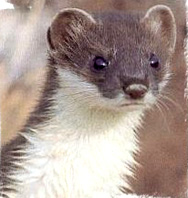
\includegraphics[width=5cm]{fouine2.jpg} }} \\
    \subfloat[Un bébé fouine]{{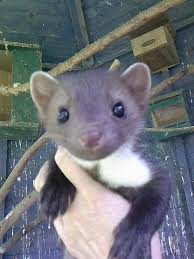
\includegraphics[width=5cm]{fouine3.jpeg} }}%
    \qquad \qquad
    \subfloat[Pas vraiment une fouine]{{
\includegraphics[width=5cm]{chat.jpeg} }}%
    \caption{Des photos de fouine trop mignonnes}
\end{figure}